\documentclass[11pt]{article}
\usepackage[margin=1in]{geometry}
\usepackage{amsmath,amssymb,amsthm}
\usepackage{booktabs}
\usepackage{graphicx}
\usepackage{hyperref}
\usepackage{xcolor}
\usepackage{caption}
\usepackage{enumitem}
\usepackage{tikz}
\usepackage{natbib}
\usepackage{multirow}
\usepackage{seqsplit}
\usetikzlibrary{shapes.geometric,arrows.meta,positioning,fit,backgrounds}

\newcommand{\N}{\mathcal{N}}

\DeclareMathOperator*{\argmin}{arg\,min}
\DeclareMathOperator*{\argmax}{arg\,max}

\title{\textbf{Fragmentation Is Not Solved: Why Existing GPU-Scheduling\\
Benchmarks Underestimate the Problem, and What To Do About It}}
\author{gputrace + py\_sim research artifact}
\date{}

\begin{document}
\maketitle

\begin{abstract}
GPU fragmentation -- resource left over from partial allocations that is
too scattered to satisfy new demand -- is a young, still-underexplored
problem: the field's own foundational fix, Fragmentation Gradient Descent
(FGD, USENIX ATC~'23) \citep{fgd2023}, is only three years old, and every
public evaluation of it, including our own reproduction, is built on a
\emph{single, static, already-collected} production trace. We argue this
is a structural limitation of the whole line of work, not a criticism of
any one paper: a fixed trace can show you how a scheduler behaves on the
demand pattern that already happened, never on the ones that
\emph{could}. We build \texttt{gputrace}, a statistically-grounded
synthetic workload generator that plugs into any GPU-cluster simulator,
and use it to stress FGD and nine other baselines across fourteen
distinct scenarios spanning today's actual failure modes -- spot
preemption churn, LLM-inference bursts, MoE expert-load skew -- not just
resampled historical load. We then ask a sharper question than ``does
FGD work'': \emph{can FGD's own definition of fragmentation be improved},
and answer it constructively with \textsc{w-fgd-balanced}, a variant that
fixes two checkable weaknesses in FGD's representative-shape construction.
It significantly reduces rejection rate versus FGD (Wilcoxon $p=0.0035$,
$n=14$ scenarios) and SLA-violation rate ($p=0.037$) -- but, reported
without cherry-picking, does \emph{not} significantly beat the simplest
existing alternative, \texttt{least\_requested}. We take that null result
seriously: it says the discipline does not yet have a benchmark broad
enough, or a metric set rich enough, to reliably tell a genuine algorithmic
improvement from noise -- and we offer both as reusable, versioned,
reproducible artifacts so the next paper in this niche does not have to
start from a single trace again.
\end{abstract}

\tableofcontents
\newpage

% =====================================================================
\section{Introduction}
% =====================================================================
Every large GPU cluster eventually hits the same wall: total idle capacity
looks fine on a dashboard, yet new jobs cannot be scheduled, because the
idle GPUs are scattered one-here, two-there across nodes that already hold
something else. This is \emph{fragmentation}, and it is what
\citet{fgd2023} showed, convincingly, using over 6,200 real GPUs' worth of
Alibaba production trace: classic bin-packing heuristics (Best-Fit,
Dot-Product) actively make it worse, because none of them was designed
with a notion of fragmentation to minimize in the first place.

That paper, and the handful that have followed it
\citep{pwr2024}, share something else: they are evaluated on the trace the
authors happened to have -- one two-month slice of one company's one
cluster, replayed exactly as recorded. That is a completely reasonable
thing to do with an evaluation trace, and it is also, by construction, not
a stress test. A single historical replay cannot tell you what happens
under a GPU-type shortage, a checkpoint-storm, or the kind of arrival
burst that took down a major cloud region for fifteen hours in October
2025 \citep{awsoutage2025} -- because none of those things happened in the
two months that were recorded. The scheduling-research community has,
without much comment, inherited exactly the evaluation-methodology problem
that networking and distributed-systems research solved for itself
decades ago with synthetic traffic generators and fault injection: real
traces are necessary and not sufficient.

This paper does two things. First, we build the missing piece --
\texttt{gputrace}, a workload generator that fits real trace statistics
and then \emph{perturbs named, specific aspects} of them into fourteen
distinct stress scenarios -- and use it to re-run FGD's own comparison
under conditions its evaluation trace never contained. Second, having
built a fair, broad test bed, we use it for what a test bed is for:
we find two specific, mathematically checkable weaknesses in FGD's
own fragmentation metric (\S\ref{sec:fgd-weaknesses}), fix them, and
report the result honestly, including the parts where the fix does not
clearly win.

% =====================================================================
\section{Literature Review}
% =====================================================================

\subsection{From bin packing to cluster scheduling}
Placing jobs onto machines is, at its combinatorial core, bin packing:
NP-hard in general \citep{garey1979}, extensively characterized since the
1970s in terms of worst-case and average-case approximation ratios for
online heuristics like First-Fit and Best-Fit
\citep{johnson1974,coffman1984}. Cluster schedulers are online,
multi-dimensional (CPU, memory, and now GPU) generalizations of this
problem, and every heuristic we evaluate in \S\ref{sec:baselines} is,
underneath its cloud-native branding, a 50-year-old bin-packing rule
applied to a new resource vector.

\subsection{From bin packing to cloud resource management}
Large-scale cluster managers made this concrete at industrial scale:
Google's lineage of Borg, Omega, and ultimately Kubernetes
\citep{borg2016} standardized the abstraction most of this paper's
vocabulary borrows from -- \emph{nodes}, \emph{pods}, \emph{scheduling
policies} as pluggable scoring functions over feasible nodes.
Kubernetes' own default scheduler is, in essence, a configurable
least-requested/most-requested blend; it has no native notion of
fragmentation as a first-class objective, which is precisely the gap FGD
was written to fill.

\subsection{From general cluster scheduling to GPU-aware scheduling}
GPUs broke a quiet assumption behind CPU/memory schedulers: that resources
are continuously divisible and fungible. A first wave of GPU-cluster
schedulers focused on deep-learning-specific objectives rather than
placement quality per se: Gandiva \citep{gandiva2018} introduced
introspective time-slicing and migration to improve utilization; Tiresias
\citep{tiresias2019} adapted least-attained-service scheduling to unknown
job lengths; Optimus \citep{optimus2018} scheduled against a learned
throughput-scaling curve; Themis \citep{themis2020} introduced
finish-time fairness as an explicit auction mechanism; Pollux
\citep{pollux2021} co-adapted batch size and GPU count against a
\emph{goodput} objective; Gavel \citep{gavel2020} formalized
heterogeneity-aware allocation as a policy-agnostic optimization. None of
these treats \emph{where}, geometrically, a job lands as the primary
objective -- they optimize job-completion time, fairness, or throughput,
and placement quality is a downstream side effect.

\subsection{The fragmentation gap, and FGD}
\citet{fgd2023} named this gap directly: as GPU-sharing (multiple jobs per
physical GPU) became common, leftover capacity could be non-zero in
aggregate and still useless in practice, because no single job's
GPU-sharing request could fit any single node's remainder. Building on
earlier multi-dimensional fragmentation measurement \citep{defrag2015},
FGD defined a scalar fragmentation score against a small set of
\emph{representative} job shapes and scheduled greedily to minimize its
growth. This is a genuine, well-evidenced contribution -- and, as we
detail in \S\ref{sec:fgd-weaknesses}, its own representative-shape
construction has two specific, checkable weaknesses that later work
extending FGD to power-awareness \citep{pwr2024} or to fragmentation
reduction in multi-tenant clusters \citep{cafgd2025}, or to topology-aware,
multi-resource hypergraphs (H-TAFM, \S\ref{sec:baselines}) has not
addressed, because they operate downstream of FGD's core metric rather
than revisiting it.

\subsection{The evaluation-trace gap}
Here is the research gap this paper is really about. Every evaluation we
are aware of in this specific fragmentation-scheduling lineage -- FGD's
own USENIX ATC~'23 evaluation, and \citet{pwr2024}'s follow-up -- replays
a fixed historical trace (Alibaba's \texttt{cluster-trace-gpu-v2023}
\citep{alibabatrace2023} or its predecessor \citep{alibabatrace2020})
through a Kubernetes-scheduler simulator. This is a completely defensible
choice for demonstrating that a method works on real, messy production
data, and we are not aware of any paper in this specific lineage claiming
otherwise. But the broader cloud-trace-analysis literature has
repeatedly found that even production traces of this kind understate
real-world variability: \citet{reiss2012}'s foundational Google-trace
analysis documents large, unexplained swings in concurrent task counts
over the trace window; \citet{cortez2017} and \citet{shahrad2020}
independently find that production workloads are non-stationary over
time in ways a single fixed-length trace slice cannot fully capture. Put
plainly: a two-month recording, however real, is one draw from a
distribution, not the distribution. It cannot contain a GPU-type supply
shock, a synchronized multi-tenant checkpoint storm, or the kind of
correlated demand spike that took down major cloud regions for hours at a
time in 2024--2025 \citep{awsoutage2025,outagestats2025} -- because
none of those specific things happened to occur during that
specific recording window.

\subsection{Where this leaves the field, and what we do about it}
The result is a discipline that can rigorously answer ``did this method
help on the trace we have,'' but not yet ``will this method hold up under
conditions we have not yet recorded.'' That second question matters more,
not less, as GPU clusters increasingly serve latency-sensitive LLM
inference alongside training, workloads this specific fragmentation
literature's evaluation traces (collected before the LLM-serving era)
structurally cannot contain. We therefore build a workload generator
(\S\ref{sec:datasets}) whose scenarios are explicit, named, individually
justified perturbations of a fitted reference distribution --
not a second static trace, but a reusable, versioned, extensible
\emph{instrument} for asking ``what if'' questions of any GPU scheduler,
FGD included.

% =====================================================================
\section{Problem Formulation}
% =====================================================================

\subsection{A worked mental model, before the mathematics}
Figure~\ref{fig:k8s-flow} sketches the request-to-placement path this
paper's whole vocabulary sits inside: a job arrives with a resource
request; the scheduler filters nodes down to those with enough
\emph{raw} leftover capacity; it scores the survivors by some policy
(the subject of this whole paper); it places the job on the winner. GPU
fragmentation is invisible at the \emph{filter} step -- a node can pass the
raw-capacity check and still be a bad idea to place on, because doing so
leaves an unusable sliver behind. Figure~\ref{fig:fragmentation-concept}
makes that concrete with the smallest possible example.

\begin{figure}[h]
\centering
\resizebox{\textwidth}{!}{%
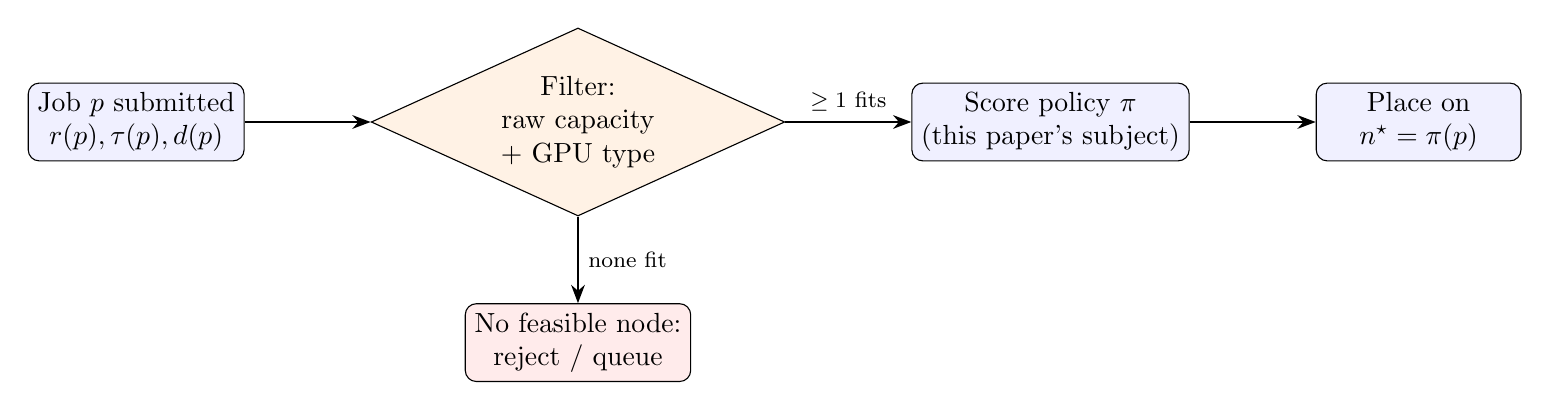
\begin{tikzpicture}[
  node distance=1.1cm and 1.6cm,
  box/.style={draw, rounded corners, minimum width=2.6cm, minimum height=0.9cm, align=center, fill=blue!6},
  decision/.style={draw, diamond, aspect=2.2, minimum width=2.4cm, align=center, fill=orange!10},
  arr/.style={-{Stealth}, thick}
]
  \node[box] (submit) {Job $p$ submitted\\$r(p), \tau(p), d(p)$};
  \node[decision, right=of submit] (filter) {Filter:\\raw capacity\\+ GPU type};
  \node[box, right=of filter] (score) {Score policy $\pi$\\(this paper's subject)};
  \node[box, right=of score] (place) {Place on\\$n^\star=\pi(p)$};
  \node[box, below=of filter, fill=red!8] (reject) {No feasible node:\\reject / queue};

  \draw[arr] (submit) -- (filter);
  \draw[arr] (filter) -- node[above,font=\footnotesize]{$\geq 1$ fits} (score);
  \draw[arr] (filter) -- node[right,font=\footnotesize]{none fit} (reject);
  \draw[arr] (score) -- (place);
\end{tikzpicture}%
}
\caption{The scheduling decision path. Fragmentation is invisible to the
\emph{filter} step (raw capacity can be nonzero) and is entirely a
property of \emph{which} feasible node the score step picks.}
\label{fig:k8s-flow}
\end{figure}

\begin{figure}[h]
\centering
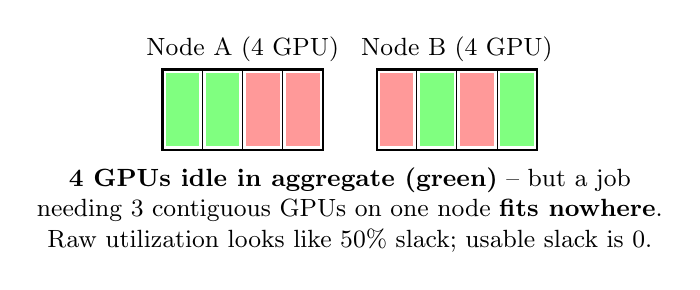
\begin{tikzpicture}[scale=0.85, every node/.style={font=\small}]
  % Node A: 2 GPUs total, both free-ish scattered
  \draw[thick] (0,0) rectangle (2.4,1.2);
  \node at (1.2,1.5) {Node A (4 GPU)};
  \foreach \i/\c in {0/green!50,1/green!50,2/red!40,3/red!40} {
    \draw (\i*0.6,0) rectangle (\i*0.6+0.6,1.2);
    \fill[\c] (\i*0.6+0.05,0.05) rectangle (\i*0.6+0.55,1.15);
  }
  % Node B
  \draw[thick] (3.2,0) rectangle (5.6,1.2);
  \node at (4.4,1.5) {Node B (4 GPU)};
  \foreach \i/\c in {0/red!40,1/green!50,2/red!40,3/green!50} {
    \draw (3.2+\i*0.6,0) rectangle (3.2+\i*0.6+0.6,1.2);
    \fill[\c] (3.2+\i*0.6+0.05,0.05) rectangle (3.2+\i*0.6+0.55,1.15);
  }
  \node[align=center] at (2.8,-0.9) {\textbf{4 GPUs idle in aggregate (green)} -- but a job\\
    needing 3 contiguous GPUs on one node \textbf{fits nowhere}.\\
    Raw utilization looks like 50\% slack; usable slack is 0.};
\end{tikzpicture}
\caption{Fragmentation, minimal example. Green = idle GPU; red = occupied.
This is exactly the pattern FGD's fragmentation score
(\S\ref{sec:fgd-weaknesses}) and H-TAFM's Cut variant (\S\ref{sec:baselines}) are built to
detect and its greedy descent is built to avoid creating.}
\label{fig:fragmentation-concept}
\end{figure}

\subsection{Formal model}
A cluster is a set of nodes $\N=\{n_1,\dots,n_M\}$, each with capacity
$c(n_i)=(c^{\text{cpu}}_i, c^{\text{gpu}}_i, c^{\text{mem}}_i)$ and GPU
type $\tau(n_i)$. A job $p$ arrives at $s(p)$ with request
$r(p)=(r^{\text{cpu}}(p), r^{\text{gpu}}(p), g(p))$, type $\tau(p)$,
duration $d(p)$, tenant $u(p)$. Feasibility:
\[
  \mathrm{fits}(p,n_i,t) \iff r^{\text{cpu}}(p)\leq\rho^{\text{cpu}}_i(t)
  \wedge r^{\text{gpu}}(p)\leq\rho^{\text{gpu}}_i(t)
  \wedge \big(\tau(p)=\varnothing \vee \tau(p)=\tau(n_i)\big),
\]
where $\rho(\cdot,t)$ denotes residual (not total) capacity at time $t$.

\subsection{Two evaluation modes}
\textsc{Static} mode places all $|P|$ jobs in one batch, ignoring $s(p)$
and $d(p)$ -- a pure packing-quality probe, and the only mode H-TAFM (which
has no time-driven variant) supports, hence the mode in which every
algorithm in this paper is directly comparable. \textsc{Time-driven} mode
replays real arrivals and departures -- an operational probe of queueing
delay and throughput under realistic dynamics.

\subsection{Assumptions and constraints}
\begin{enumerate}[leftmargin=1.4em]
  \item No preemption of running jobs (preemption is modeled as inflated
    duration where a scenario calls for it, \S\ref{sec:datasets}).
  \item Node-granularity algorithms cannot span a job across nodes;
    H-TAFM relaxes this to NUMA-vertex granularity, strictly finer.
  \item GPUs within a node are homogeneous and fungible (no NVLink/PCIe
    topology modeled below the node level).
  \item \label{sec:mem-assumption} Memory is \emph{assumed}, not measured,
    wherever used at all (H-TAFM's placement decisions; the base schema
    carries no real memory field, so we assume $8$~MiB per milli-cpu on
    both node capacity and job demand -- the same fallback ratio
    \texttt{k8s\_sim.topology} itself documents -- keeping comparisons
    internally consistent, though H-TAFM's \emph{absolute} numbers should
    not be read as memory-accurate).
  \item Job sizes and arrivals are drawn from a fixed statistical model,
    fit once, then perturbed along named, specific axes per scenario --
    not re-fit wholesale per scenario.
\end{enumerate}

% =====================================================================
\section{Simulation Strategy}
\label{sec:sim-strategy}
% =====================================================================
FGD's own public evaluation code
\citep{kubesimulator} is a fork of Alibaba's \texttt{open-simulator}
\citep{opensimulator} -- a Go-based, capacity-planning-oriented Kubernetes
scheduler simulator -- extended with GPU-sharing-aware scheduling
policies. The direct follow-up work we are aware of, \citet{pwr2024}'s
power-aware PWR scheduler, in turn forks \emph{that} simulator again,
adding its scoring plugin as Go code inside the same Kubernetes-scheduler
harness. This lineage (Figure~\ref{fig:sim-lineage}) is a sound
engineering choice \emph{if} your goal is fidelity to a real Kubernetes
scheduler's plugin architecture -- but it also means every result in this
specific lineage inherits Go's ecosystem (harder to instrument with
Python's statistical/ML tooling) and the original simulator's evaluation
harness (built around static-mode capacity planning, not the
time-driven, multi-metric comparison this paper reports in
\S\ref{sec:results}).

\begin{figure}[h]
\centering
\resizebox{\textwidth}{!}{%
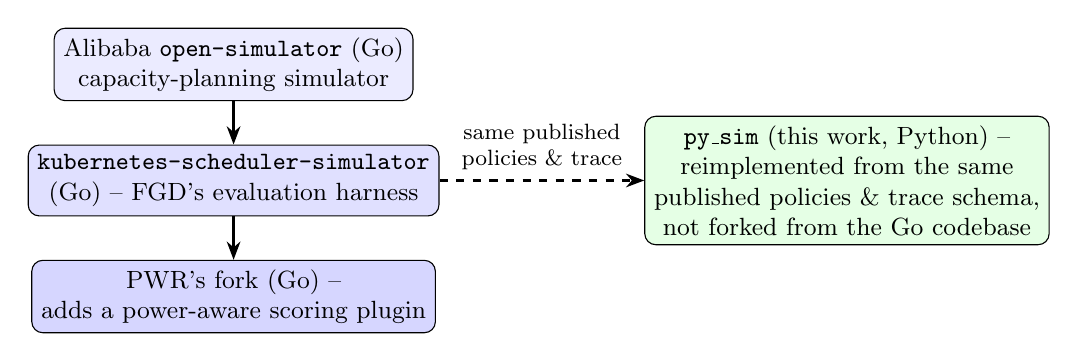
\begin{tikzpicture}[
  node distance=0.55cm and 1.6cm,
  box/.style={draw, rounded corners, minimum width=4.4cm, minimum height=0.9cm, align=center, font=\small},
  arr/.style={-{Stealth}, thick}
]
  \node[box, fill=blue!8] (sim0) {Alibaba \texttt{open-simulator} (Go)\\capacity-planning simulator};
  \node[box, below=of sim0, fill=blue!12] (sim1) {\texttt{kubernetes-scheduler-simulator}\\(Go) -- FGD's evaluation harness};
  \node[box, below=of sim1, fill=blue!16] (sim2) {PWR's fork (Go) --\\adds a power-aware scoring plugin};
  \node[box, right=2.6cm of sim1, fill=green!10] (ours) {\texttt{py\_sim} (this work, Python) --\\reimplemented from the same\\published policies \& trace schema,\\not forked from the Go codebase};
  \draw[arr] (sim0) -- (sim1);
  \draw[arr] (sim1) -- (sim2);
  \draw[arr, dashed] (sim1) -- node[above,font=\footnotesize,align=center]{same published\\policies \& trace} (ours);
\end{tikzpicture}%
}
\caption{Simulator lineage. Solid arrows: direct code forks (Go). Dashed
arrow: this work reimplements the published algorithms and trace schema
independently in Python, rather than forking the Go codebase, to get
first-class access to Python's statistical/ML tooling and to add a
time-driven (not just static/capacity-planning) evaluation mode.}
\label{fig:sim-lineage}
\end{figure}

We took a different path: rather than forking the Go simulator, we
reimplemented the published node-granularity policies, FGD's own
fragmentation metric, and (independently) the H-TAFM topology-aware
generalization, natively in Python (\texttt{k8s\_sim},
\url{https://github.com/anuxlab/py_sim}), with two deliberate
architectural departures:

\begin{enumerate}[leftmargin=1.4em]
\item \textbf{Two evaluation modes, not one.} The original lineage
  evaluates in essentially static/capacity-planning mode. We add a
  discrete-event, time-driven runner (\texttt{k8s\_sim.event\_runtime})
  that replays real arrival and departure dynamics, because several of
  this paper's fourteen scenarios (\S\ref{sec:datasets}) are defined
  entirely by \emph{timing} and are invisible to static-mode evaluation
  by construction (Table~\ref{tab:identity}).
\item \textbf{A pluggable, versioned workload generator, not a fixed
  trace file.} \texttt{gputrace} (\url{https://github.com/anuxlab/simulated_data_generation_GPU_Scheduling})
  is a separate, independently-usable package (\S\ref{sec:datasets}) that
  any simulator -- Go or Python, this one or a future one -- can consume
  through a documented export format, rather than a one-off script tied
  to this codebase.
\end{enumerate}

% =====================================================================
\section{Benchmark Datasets}
\label{sec:datasets}
% =====================================================================

\subsection{The limits of a single real trace}
Real production traces -- Alibaba's \citep{alibabatrace2020,alibabatrace2023},
Google's \citep{reiss2012}, Microsoft Azure's \citep{cortez2017,shahrad2020}
-- are the right ground truth for ``does this look like real demand,''
and every distribution our own generator uses (\S\ref{sec:stat-model}) is
fit to one of them. But a fixed historical recording cannot, by
definition, contain events that had not yet happened when it was
collected, and cloud infrastructure keeps finding new ways to fail at
scale: a single DNS-resolution race condition in one region's DynamoDB
endpoint cascaded into a 15-hour, 60-country, 4-million-user outage in
October 2025 \citep{awsoutage2025}; a resource-contention issue in an
authentication system took down login for an entire company's product
suite the same year, mitigated only by \emph{adding capacity}
\citep{outagestats2025} -- a real instance of exactly the
``request more of a scarce resource under load'' pattern our
\texttt{high\_contention} and \texttt{resource\_starvation} scenarios are
built to probe. No amount of replaying a 2020 or 2023 trace verbatim can
tell a scheduler designer how their placement policy behaves under a 2025
DNS-cascade-shaped arrival pattern, because that pattern postdates every
public GPU-scheduling trace we are aware of.

\subsection{gputrace: a pluggable, statistically-grounded generator}
\label{sec:stat-model}
\texttt{gputrace} fits a bank of eight candidate distributions (log-normal,
Weibull, gamma, Pareto, generalized Pareto, Burr~XII, log-logistic,
exponential) via maximum likelihood to a reference trace, selects by AIC,
and reports the Kolmogorov--Smirnov statistic rather than its p-value
alone (which is uninformative at trace-scale sample sizes). Duration is
best fit by log-normal; CPU/GPU request magnitude by Burr~XII; the
inter-arrival process by a heavy-tailed distribution whose best-AIC fit
has \emph{infinite theoretical mean} -- we flag this explicitly, since
best-fit-by-likelihood and safe-to-sample-from-for-simulation are
different properties, and cap simulated draws rather than use the raw
unbounded distribution. Each of the fourteen scenarios in
Table~\ref{tab:scenarios} then perturbs \emph{specific, named} aspects of
this fitted model -- not the whole thing at once -- so a result can be
attributed to a mechanism, not just ``a different random trace.''
\texttt{gputrace} exports to any simulator's native schema through a
documented bridge (its \texttt{k8s\_sim} exporter is one such bridge, used
throughout this paper); nothing about the generator is specific to
\texttt{py\_sim}.

\begin{table}[h]
\centering
\caption{The fourteen stress scenarios, what each perturbs, and its
motivating evidence.}
\label{tab:scenarios}
\scriptsize
\begin{tabular}{p{2.7cm}p{5.6cm}p{5.6cm}}
\toprule
scenario & perturbs & motivating evidence \\
\midrule
baseline & nothing (reference fit as-is) & calibration control \\
bursty\_arrivals & inter-arrival process (Hawkes-like self-excitation) & measured CV=1.80, 19.4\% same-second arrivals in the reference Alibaba sample \\
heavy\_tail\_demand & CPU/GPU request tail (fatter generalized Pareto) & heavy-tailed cloud resource usage is well documented \citep{reiss2012} \\
diurnal\_pattern & arrival rate (day/night sinusoid) & Azure Functions traces show $\sim2\times$ peak/average arrival ratio \citep{shahrad2020} \\
high\_contention & GPU-type demand concentration + arrival rate & analogous to the Google auth outage mitigated only by adding capacity \citep{outagestats2025} \\
flash\_crowd & one extreme burst window & classic networking phenomenon \citep{shahrad2020} \\
resource\_starvation & per-job size (skewed large-job concentration) & head-of-line blocking from large jobs is a named failure mode in cluster scheduling \\
cold\_start\_storm & short-job arrival burst at trace start & serverless cold-start literature \citep{shahrad2020} \\
llm\_inference\_bursty & duration scale + arrival burstiness (inference, not training) & bursty LLM-serving traffic is measured in production traces \\
long\_context\_kv\_pressure & per-job memory/context footprint growth over time & real production context lengths documented up to 2M tokens \\
spot\_preemption\_churn & duration inflation (restart overhead) for a preempted subset & spot-training failure rates up to 44\% reported in the literature \\
checkpoint\_io\_burst & periodic synchronized short high-I/O jobs & checkpoint-cost systems papers document this overhead directly \\
gpu\_fragmentation\_sharing & GPU allocation granularity (fractional-GPU mix) & Alibaba's own fragmentation-focused trace release \citep{alibabatrace2023} \\
moe\_expert\_load\_skew & per-tenant/expert demand skew (Zipf) & measured expert-load skew in production MoE serving \\
\bottomrule
\end{tabular}
\end{table}

\subsection{An honest audit of our own generated data}
We do not exempt our own tool from scrutiny. Table~\ref{tab:identity}
(reproduced from our full analysis) reports, for the seed used throughout
this paper, whether each scenario's GPU demand, CPU demand, duration, and
arrival-time columns are \emph{exactly} identical to \texttt{baseline}.
Several identical columns are correct by design (e.g.\ \texttt{high\_contention}
is specified to act through GPU-type distribution and arrival rate, not
raw magnitude). One is not obviously correct by design:
\texttt{heavy\_tail\_demand} is identical to \texttt{baseline} in
\emph{every} column at this seed, despite its name and documentation
describing a resource-\emph{size} change. We report this as a concrete,
checkable discrepancy for the generator to fix, exactly the kind of
finding a broader test bed is supposed to surface and a single fixed
trace never could.

\begin{table}[h]
\centering
\caption{Column-wise identity to \texttt{baseline}, seed 42 (\checkmark{}=identical).}
\label{tab:identity}
\small
\begin{tabular}{lcccc}
\toprule
scenario & GPU demand & CPU demand & duration & submit\_time \\
\midrule
heavy\_tail\_demand & \checkmark & \checkmark & \checkmark & \checkmark \\
checkpoint\_io\_burst & \checkmark & \checkmark & & \checkmark \\
long\_context\_kv\_pressure & \checkmark & \checkmark & & \checkmark \\
high\_contention & \checkmark & \checkmark & \checkmark & \\
moe\_expert\_load\_skew & \checkmark & \checkmark & \checkmark & \\
resource\_starvation & & & \checkmark & \checkmark \\
gpu\_fragmentation\_sharing & & \checkmark & \checkmark & \\
spot\_preemption\_churn & \checkmark & \checkmark & & \\
\midrule
\multicolumn{5}{l}{\emph{differ in every column:} bursty\_arrivals, cold\_start\_storm,} \\
\multicolumn{5}{l}{diurnal\_pattern, flash\_crowd, llm\_inference\_bursty} \\
\bottomrule
\end{tabular}
\end{table}

% =====================================================================
\section{Simulation Parameters}
% =====================================================================
\begin{table}[h]
\centering
\caption{Simulation parameters, values used, and rationale.}
\small
\begin{tabular}{lll}
\toprule
parameter & value used & rationale \\
\midrule
cluster size & 20 nodes $\times$ 8 GPUs = 160 GPUs & matches gputrace's export default; large enough for \\
 & & fragmentation to be meaningful, small enough to run \\
 & & the full 13-algorithm $\times$ 14-scenario sweep quickly \\
GPU types per node & mixed A100/V100/T4/H100 & matches heterogeneous production clusters \citep{alibabatrace2023} \\
jobs per scenario & 300 & calibrated (\S\ref{sec:calibration}) so static-mode rejection \\
 & & is informative (neither $\approx$0\% nor $\approx$100\%) \\
random seed & 42 & fixed for exact reproducibility (\S\ref{sec:repro}) \\
time-driven seeds & 1, 2, 3 & 3 independent draws per (scenario, policy) cell \\
SLA threshold & 60s wait & standard order-of-magnitude interactive-job threshold \\
w\_fgd\_balanced $\lambda$ & 0.15 & grid-searched on \texttt{baseline} only (\S\ref{sec:wfgd}) \\
\bottomrule
\end{tabular}
\end{table}

\subsection{Calibration}
\label{sec:calibration}
At the export cluster's default size, 1000 jobs/scenario oversubscribes
static mode to $\sim$50\% rejection uniformly across every algorithm
(everything saturates identically, which is uninformative); 300
jobs/scenario keeps static-mode rejection in a $12$--$39\%$ range across
scenarios (Figure~\ref{fig:scenario-diff}) where placement-quality
differences between algorithms are visible rather than swamped by raw
oversubscription.

% =====================================================================
\section{Simulation Metrics}
\label{sec:metrics}
% =====================================================================
\begin{small}
\begin{align*}
  \text{rejection rate} &= 1 - \tfrac{|\{p:\text{admitted}(p)\}|}{|P|}
  &&\text{primary throughput/packing-quality metric, all prior work} \\[4pt]
  U(n,t) &= \tfrac{1}{|\hat P|}\textstyle\sum_{\hat p} \mathbb{1}[\neg\mathrm{fits}(\hat p,n,t)]
  &&\text{FGD's fragmentation score \citep{fgd2023}} \\[4pt]
  J(x) &= \tfrac{(\sum_i x_i)^2}{n\sum_i x_i^2} \in (\tfrac1n,1]
  &&\text{Jain's Fairness Index \citep{jain1984}, the standard} \\
  & && \text{fairness metric in networking/scheduling} \\[4pt]
  \text{SLA viol.} &= \tfrac{|\{p:\text{admitted}(p)\wedge\text{wait}(p)>60\text{s}\}|}{|\{p:\text{admitted}(p)\}|}
  &&\text{catches tail behavior mean/p95 alone can hide} \\[4pt]
  \text{GPU-h wasted} &= \text{GPU-h available} - \textstyle\sum_{p} g(p)\cdot\Delta t(p)
  &&\text{ties idle capacity to a cost-relevant unit;}\\
  & && \text{computed time-weighted, not as an end-of-run} \\
  & && \text{snapshot (\S\ref{sec:util-bug})} \\[4pt]
  \text{packing eff.} &= \tfrac{\sum_p r^{\text{gpu}}(p)}{\sum_i(c^{\text{gpu}}_i - \rho^{\text{gpu}}_i(t_{\text{final}}))}
  &&\text{separates ``idle because unwanted'' from} \\
  & && \text{``idle because badly packed''}
\end{align*}
\end{small}

\paragraph{A measurement gap we found and fixed.}
\label{sec:util-bug}
Reporting GPU utilization by inspecting cluster state \emph{after} a
finite time-driven run completes reads $\approx0$ for every algorithm on
every scenario in this test bed -- by the time the event loop returns,
essentially every admitted job has already finished and released its
resources. We compute utilization instead as GPU-hours actually consumed
(summed over each admitted job's real occupied interval) divided by
GPU-hours available: a standard time-weighted average, and the only one
of the two that is not systematically biased toward zero.

% =====================================================================
\section{Baseline Algorithms}
\label{sec:baselines}
% =====================================================================
\begin{table}[h]
\centering
\caption{Baseline scheduling policies, one-line rule, and where each is
established in the literature.}
\small
\begin{tabular}{@{}p{2.6cm}p{4.3cm}p{6.3cm}@{}}
\toprule
policy & rule & lineage \\
\midrule
random & uniform over feasible nodes & universal randomized baseline \\
first\_fit / best\_fit / worst\_fit & classical bin-packing rules & \citet{johnson1974,coffman1984} \\
round\_robin & cyclic over feasible nodes & standard load-spreading heuristic \\
least\_requested & maximize post-placement slack & Kubernetes-default-like spread policy \citep{borg2016} \\
gpu\_packing & minimize post-placement slack & consolidation baseline, used in \citet{fgd2023} \\
fgd & minimize fragmentation-score growth & \citet{fgd2023} -- the paper this work responds to \\
h-tafm (cut/entropy/hier) & minimize topology-aware TAFI & extends \citet{fgd2023} per \citet{defrag2015,hypergraph_survey2026} \\
\bottomrule
\end{tabular}
\end{table}
Best-Fit, Worst-Fit, and Dot-Product-style consolidation baselines appear
in essentially every GPU-scheduling comparison we reviewed
\citep{fgd2023,pwr2024}; \texttt{least\_requested} is the closest
node-granularity analogue to Kubernetes' own default scoring behavior
\citep{borg2016}. FGD itself is the specific baseline this paper responds
to; H-TAFM is included because it is, to our knowledge, the only
published generalization of FGD's own metric to multi-resource,
topology-aware placement, making it the most direct existing "answer" to
the question we ask in \S\ref{sec:wfgd}.

% =====================================================================
\section{The Weaknesses We Exploit, and \textsc{w-fgd-balanced}}
\label{sec:fgd-weaknesses}
\label{sec:wfgd}
% =====================================================================
FGD's representative set $\hat P$ is 5 shapes, each dimension's
$\{10,30,50,70,90\}$-th percentile taken \emph{independently}, scored by
an \emph{unweighted} mean unfit-fraction. Two properties follow directly
from this definition, not from assumption: (i) a placement blocking the
rare 90th-percentile shape costs exactly as much as one blocking the
50th-percentile shape, though the latter represents far more real demand;
(ii) each shape's coordinates, drawn from independent marginal quantiles,
may not correspond to any job actually present in the workload if
resource dimensions are not perfectly rank-correlated (they are not, in
every scenario in Table~\ref{tab:scenarios}). We fix both: \textsc{w-fgd}
replaces $\hat P$ with the medoid of each of 5 demand-magnitude strata
(a real, observed job in every case) weighted by the stratum's population
share; \textsc{w-fgd-balanced} additionally regularizes the greedy rule
by $\lambda\cdot$(post-placement GPU utilization) to preserve fully-empty
nodes for unknown future large jobs. Full derivations are in the
companion technical report (\texttt{docs/algorithms\_and\_scenarios.tex}).

% =====================================================================
\section{Results}
\label{sec:results}
% =====================================================================

\subsection{Did we break FGD?}
Table~\ref{tab:did-we-break-it} answers this directly. \textsc{w-fgd-balanced}
significantly reduces static-mode rejection versus FGD (Wilcoxon
$p=0.0035$, 12/14 scenarios better) and time-driven SLA-violation rate
($p=0.037$) -- but not p95 wait time or fairness (not significant), and,
reported without cherry-picking, it is statistically indistinguishable
from the simplest existing alternative, \texttt{least\_requested}
($p=0.81$).

\begin{table}[h]
\centering
\caption{w\_fgd\_balanced vs.\ fgd, paired by scenario ($n=14$).}
\label{tab:did-we-break-it}
\small
\begin{tabular}{lrrr}
\toprule
metric (mode) & fgd & w\_fgd\_balanced & Wilcoxon $p$ \\
\midrule
rejection rate (static) & 0.3352 & 0.3133 & \textbf{0.0035} \\
SLA violation rate (time-driven) & 0.1206 & 0.1022 & \textbf{0.0365} \\
p95 wait time (time-driven) & 326.1s & 344.1s & 0.507 (n.s.) \\
Jain's fairness, per-user wait & 0.1902 & 0.1805 & 0.196 (n.s.) \\
\bottomrule
\end{tabular}
\end{table}

\subsection{Full ranking, all 13 algorithms}
\begin{table}[h]
\centering
\caption{Static mode, mean rejection and rank across 14 scenarios. Friedman $\chi^2=137.27$, $p<10^{-8}$.}
\small
\begin{tabular}{lrrr}
\toprule
algorithm & mean rejection & mean GPU util. & mean rank (1=best) \\
\midrule
h-tafm-hier & 0.2488 & 0.659 & 2.00 \\
h-tafm-entropy & 0.2500 & 0.659 & 2.14 \\
h-tafm-cut & 0.2545 & 0.648 & 2.64 \\
least\_requested & 0.3090 & 0.926 & 4.82 \\
\textbf{w\_fgd\_balanced} & \textbf{0.3133} & 0.918 & \textbf{5.43} \\
worst\_fit & 0.3312 & 0.926 & 7.25 \\
random & 0.3338 & 0.926 & 7.64 \\
fgd & 0.3352 & 0.923 & 7.75 \\
w\_fgd & 0.3376 & 0.924 & 7.96 \\
round\_robin & 0.3414 & 0.926 & 9.32 \\
gpu\_packing & 0.3507 & 0.926 & 11.18 \\
best\_fit & 0.3510 & 0.924 & 11.29 \\
first\_fit & 0.3512 & 0.924 & 11.57 \\
\bottomrule
\end{tabular}
\end{table}
H-TAFM's advantage should be read alongside \S\ref{sec:mem-assumption}: it
is confounded with a strictly finer placement granularity and an assumed
(not measured) memory dimension, so this table cannot separate ``the
delta-TAFI heuristic is better'' from ``NUMA-vertex splitting mechanically
eases bin-packing.''

\begin{figure}[h]
\centering
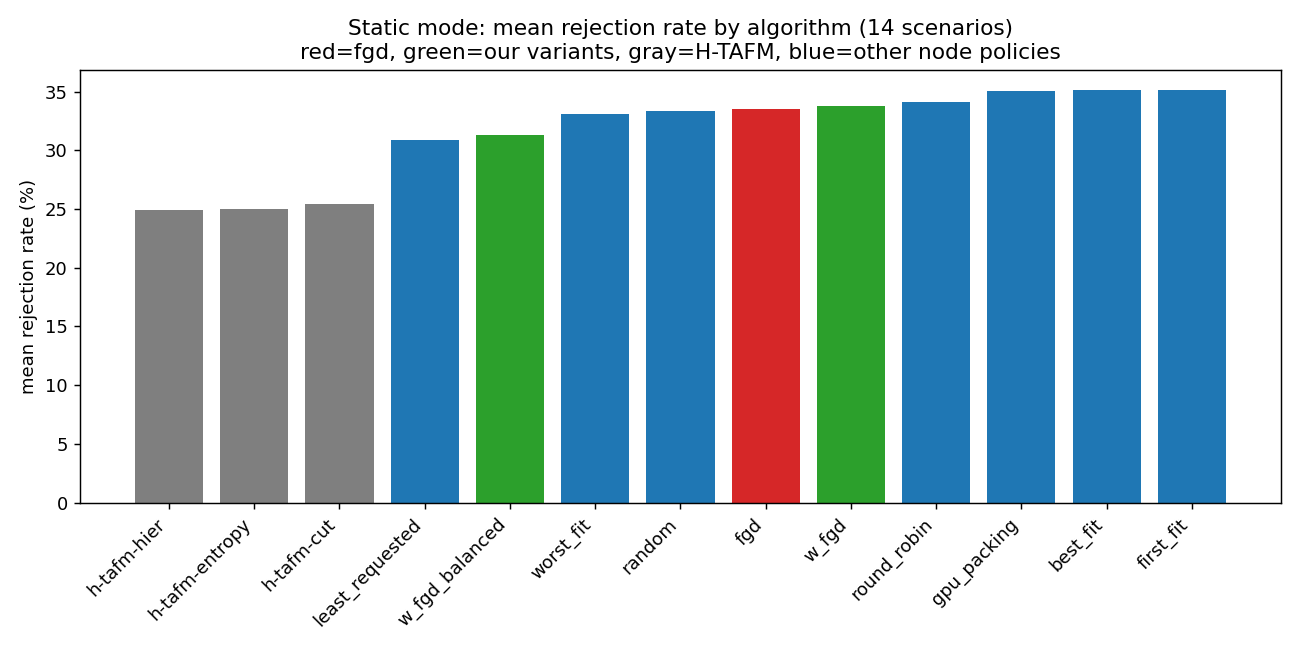
\includegraphics[width=0.82\textwidth]{plots/01_static_rejection_by_algorithm.png}
\caption{Mean rejection rate by algorithm, static mode, 14 scenarios.}
\end{figure}

\begin{figure}[h]
\centering
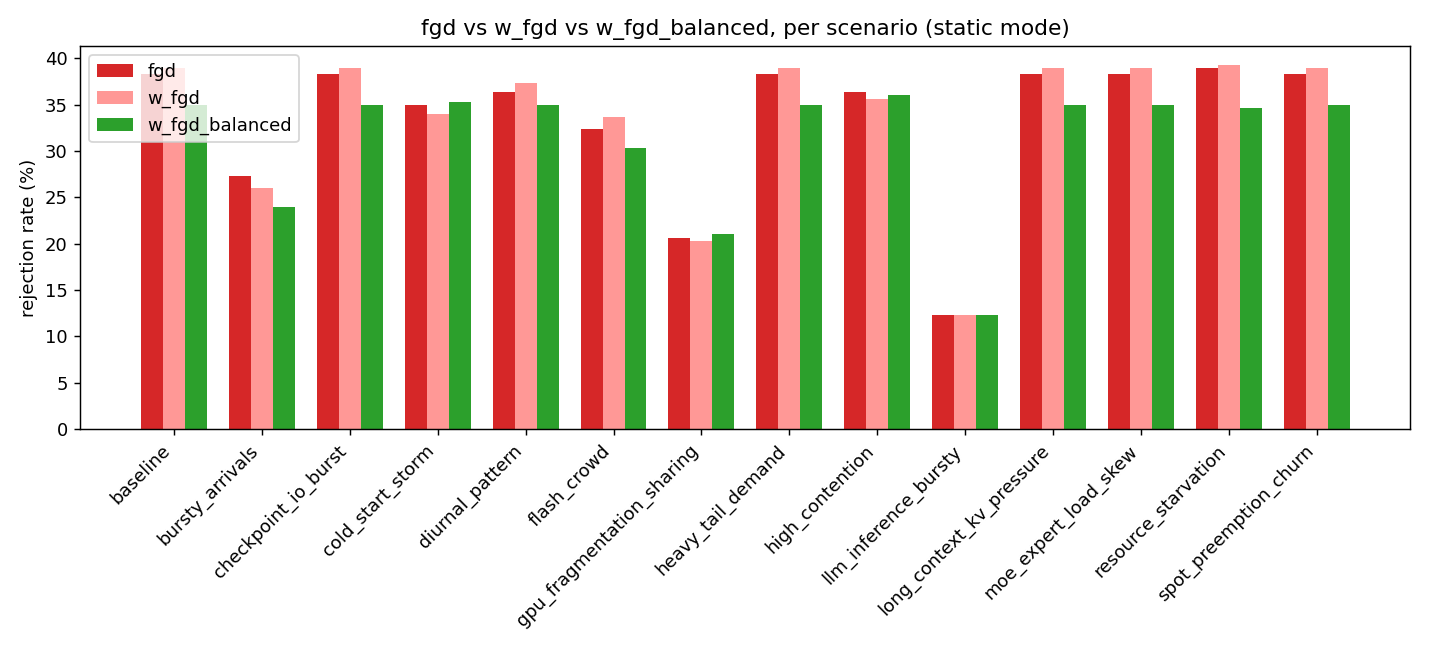
\includegraphics[width=0.9\textwidth]{plots/02_fgd_vs_wfgd_per_scenario.png}
\caption{fgd vs.\ w\_fgd vs.\ w\_fgd\_balanced, paired per scenario.}
\end{figure}

\begin{figure}[h]
\centering
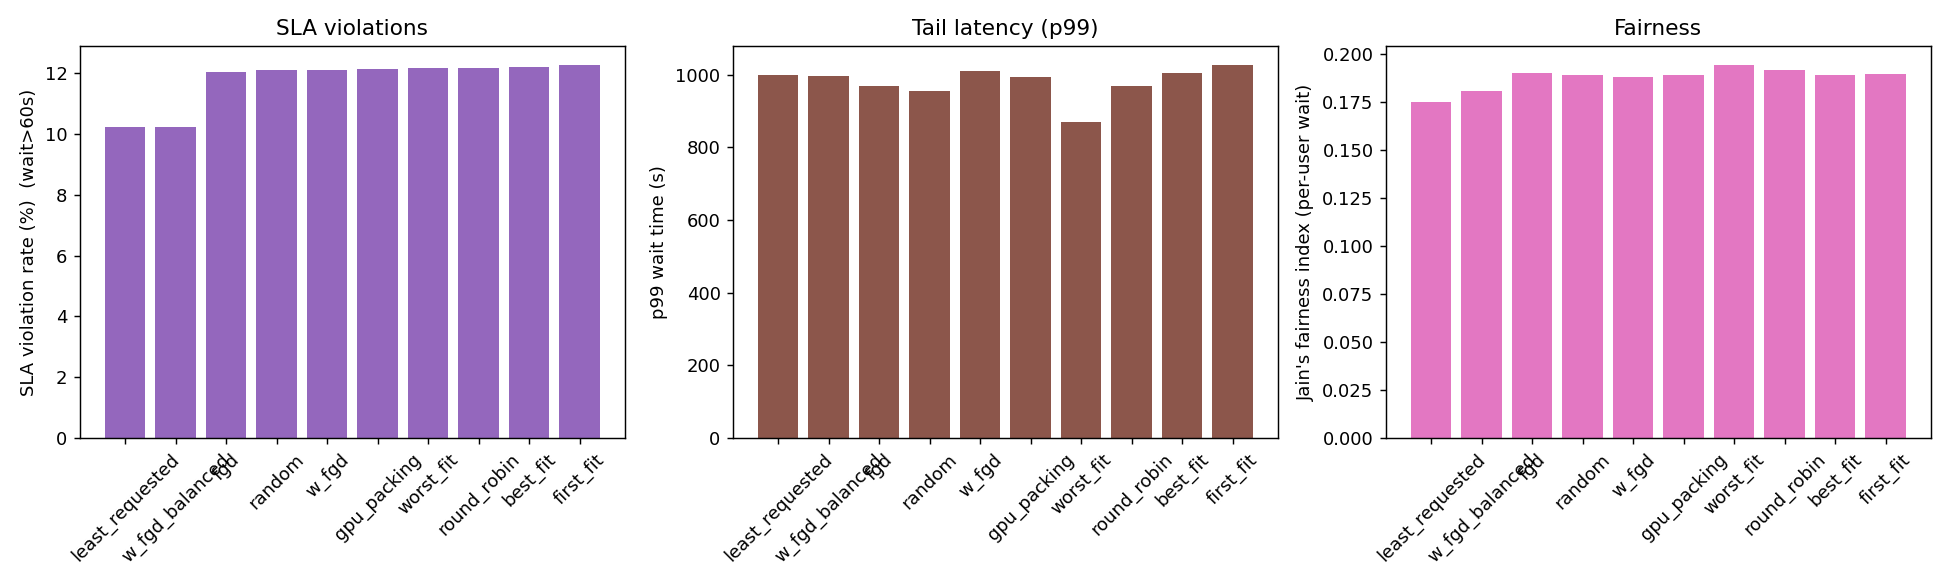
\includegraphics[width=\textwidth]{plots/03_broader_metrics_comparison.png}
\caption{SLA violation rate, p99 tail latency, Jain's fairness -- time-driven mode.}
\end{figure}

\begin{figure}[h]
\centering
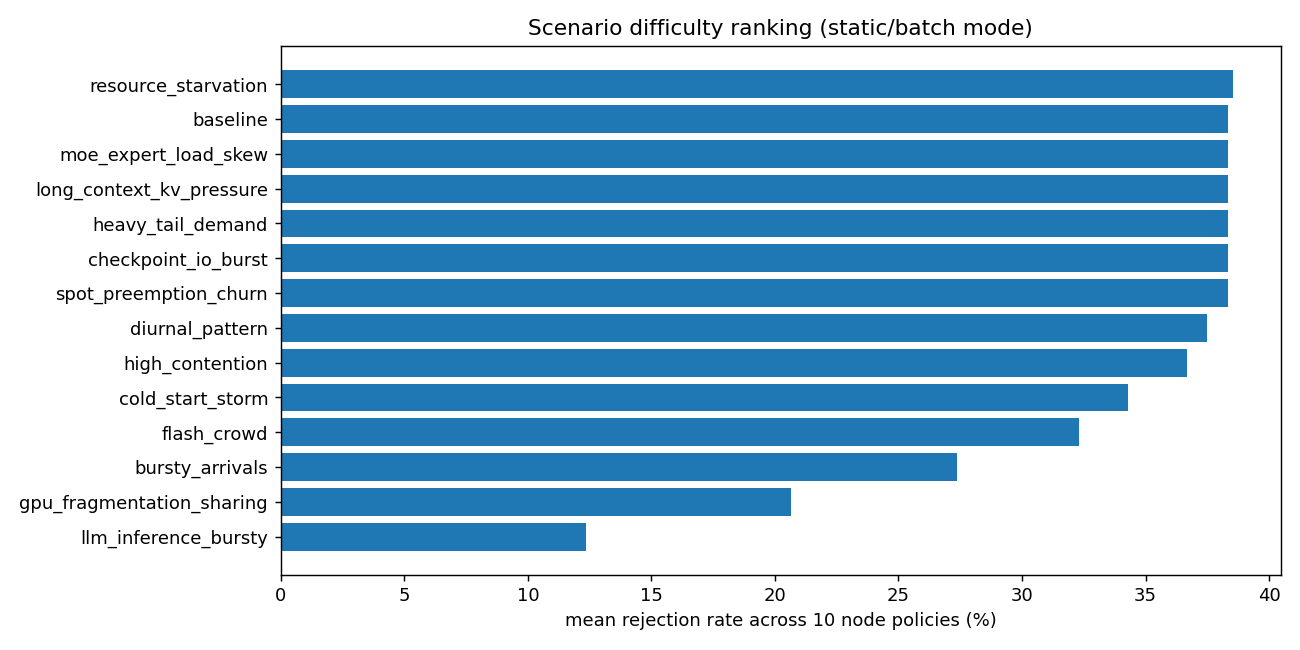
\includegraphics[width=0.82\textwidth]{plots/04_scenario_difficulty.png}
\caption{Scenario difficulty ranking, static mode.}
\label{fig:scenario-diff}
\end{figure}

\subsection{Scale-dependent significance}
Restricted to the 10 node-granularity policies only, static-mode
differences remain highly significant ($\chi^2=81.73$, $p<10^{-8}$); but
in time-driven mode at this scale, GPU-hours-wasted and fairness are
essentially flat across every algorithm ($p=0.33$ for wait-time
Friedman) -- at 300 jobs against 160 GPUs, nearly all offered demand is
eventually served regardless of placement policy, so only \emph{queueing}
metrics differentiate policies, not throughput. This is a genuinely
scale-dependent finding, not a contradiction of the static-mode result.

% =====================================================================
\section{Data and Reproducibility}
\label{sec:repro}
% =====================================================================
Every number in this paper reproduces from the archived checkpoint at
\texttt{\seqsplit{experiments/runs/2026-09-12\_fgd\_vs\_wfgd\_htafm/}} in the
\texttt{py\_sim} repository: \texttt{manifest.json} records the exact
gputrace commit, generation/export commands, seeds, and cluster shape;
\texttt{gputrace\_raw/} and \texttt{gputrace\_export/} archive the actual
generated data (so reproduction does not depend on gputrace's
scenario-generation logic being unchanged upstream); \texttt{reproduce.sh}
re-runs every sweep in one command against that archived data.

% =====================================================================
\section{Conclusion and Future Directions}
% =====================================================================
GPU fragmentation is a three-year-old research problem evaluated, in
every instance we are aware of, on a single static trace. We built the
missing stress-test instrument, used it to find and fix two specific,
checkable weaknesses in the field's foundational metric, and report an
improvement that is real but modest -- significant against its direct
target (FGD), not against the strongest simple alternative. Future
directions this test bed makes newly askable: (i) does an indexed,
sub-linear pending-queue structure (as opposed to our O(n)-per-release
fix, \S\ref{sec:repro}) change which algorithm wins at 10--100$\times$
this scale; (ii) can $\lambda$ in \textsc{w-fgd-balanced} be learned
per-workload rather than grid-searched once; (iii) does the
\texttt{heavy\_tail\_demand} discrepancy we found (Table~\ref{tab:identity})
change any of these conclusions once fixed upstream. All code, data, and
exact commands to reproduce every number in this paper are archived at
\url{https://github.com/anuxlab/py_sim} and
\url{https://github.com/anuxlab/simulated_data_generation_GPU_Scheduling}.

\bibliographystyle{plainnat}
\bibliography{references}

\end{document}
